\section{Verification of the Model}

To verify the model in simulation \eqref{FrameEq4TaylerApprox} is transformed into the Laplace domain, after which a transfer function of the system is derived. The proceeding equations are valid only around the operating point, and so for better overview, in the following \si{\Delta \theta_F = \theta_F}.
%
\begin{flalign}
	\eq{(J_F+m_w \cdot {l_w}^{2}) \cdot \theta_F \cdot s^2}{-B_F \theta_F\cdot s +  ( m_F \cdot l_F + m_w \cdot l_w ) g \cdot \theta_F - \tau_m + B_w \theta_w\cdot s } & \nonumber\\
\label{LaplaceOfLinearizedModel}
\end{flalign}
%
The angle of the reaction wheel, \si{\theta_w}, still features in \eqref{LaplaceOfLinearizedModel}. It is desireable to have only one input, \si{\tau_m}, and one output, \si{\theta_F}. To achieve this, \eqref{WheelRotEq2} is transformed into the Laplace domain and solved for \si{\theta_w}.
%
\begin{flalign}
	\eq{\theta_w\cdot s^2} {\frac{\tau_m - B_w \theta_w\cdot s}{J_w} - \theta_F\cdot s^2}   &\\
	\eq{\theta_w} {\frac{ -J_w \theta_F \cdot s^2 + \tau_m }{ J_w \cdot s^2 + B_w \cdot s }}&
\label{WheelRotEq2Laplace}
\end{flalign}
%
\Eqref{WheelRotEq2Laplace} is now substituted for \si{\theta_w} in \eqref{LaplaceOfLinearizedModel}, and the transfer function is of the system is derived.
%
\begin{flalign}
	\eqOne{(J_F+m_w \cdot {l_w}^{2}) \cdot \theta_F \cdot s^2}{-B_F \theta_F\cdot s +  ( m_F \cdot l_F + m_w \cdot l_w ) g \cdot \theta_F - \tau_m}
	\eqTwo{+ B_w ( \frac{ -J_w \theta_F \cdot s^2 + \tau_m }{ J_w \cdot s^2 + B_w \cdot s } )\cdot s }&\nonumber
\label{CubliTransferFunction}
\end{flalign}

\vspace{-.2cm}
\large{\si{\frac{\theta_F}{\tau_m} =}}\nolinebreak
\Large{
\si{\frac{\frac{s}{-J_F - m_w \cdot {l_w}^2}}{s^3 + \left( \frac{B_w}{J_w} + \frac{B_w + B_F}{J_F + m_w \cdot {l_w}^2} \right) s^2 - \left( \frac{ \left( m_F \cdot l_F + m_w \cdot l_w \right)\cdot g}{ \left( J_F + m_w \cdot {l_w}^2 \right) J_w} - \frac{B_F B_w}{ \left(J_F + m_w \cdot {l_w}^2 \right) J_w} \right) s - \frac{\left(m_F \cdot l_F + m_w \cdot l_w \right) B_w\cdot g}{\left(J_F + m_w \cdot {l_w}^2 \right) J_w} }}}\normalsize\vspace{-1.9cm}\\
\vspace{1.8cm}\begin{flalign}\label{2ndCubliTransferFunction}\end{flalign}
%
The transfer function from \eqref{2ndCubliTransferFunction} can be represented as well in the form of a block diagram, as seen in \figref{cubliSimulink}.
%
\begin{figure}[H] 
	\centering 
	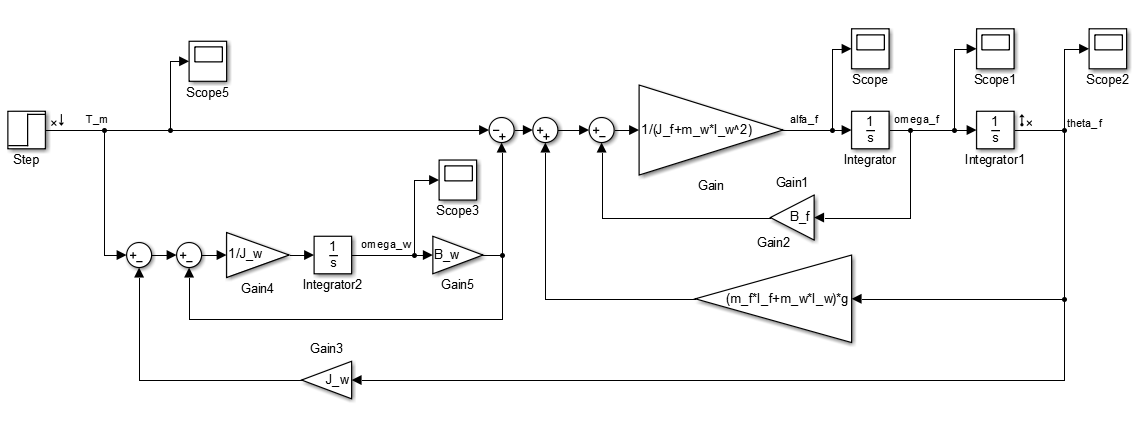
\includegraphics[scale=0.53]{figures/cubliSimulink}
	\centering
	\captionsetup{justification=centering}
	\caption{Block diagram of the system}
	\label{cubliSimulink}
\end{figure} 
%
Substituting all the constants of \eqref{2ndCubliTransferFunction} with the parameters of the real model results in the final transfer function of the system.
%
\begin{flalign}
	\eq{G(s)}{\frac{-211.9 \cdot s}{s^3 + 1.32 \cdot s^2 - 98.98 \cdot s - 2.803}} &\nonumber\\
	\label{RealCubliTransferFunction}	
\end{flalign}
%
Using \eqref{RealCubliTransferFunction} it is possible to simulate the response of the system to a step input and compare it with the response of the simulation of the block diagram. This is done to verify that the block diagram is in fact showing the system described in \eqref{RealCubliTransferFunction}.
%
\begin{figure}[H] 
	\centering 
	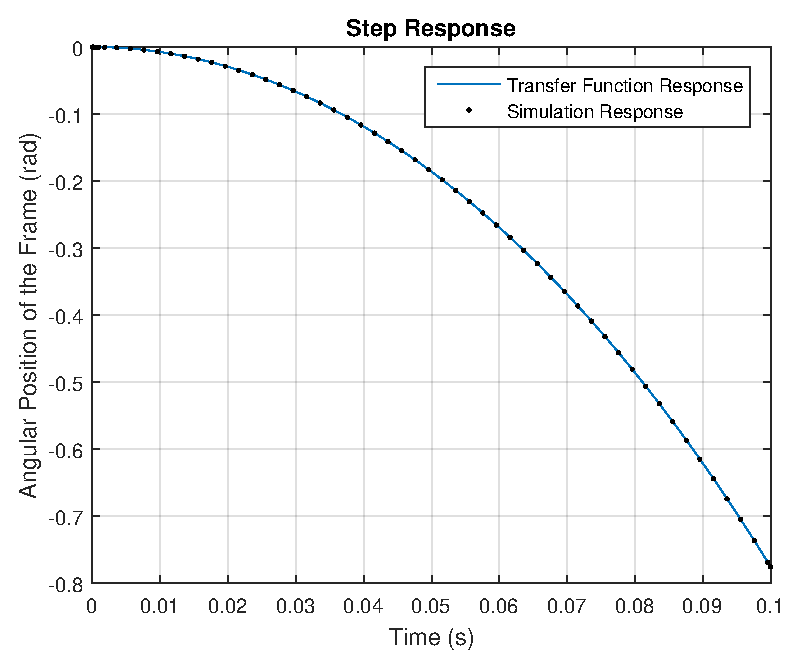
\includegraphics[scale=0.55]{figures/stepComparison}
	\centering
	\captionsetup{justification=centering}	
	\caption{Step response comparison between the transfer function from \eqref{RealCubliTransferFunction} and the block diagram from \figref{cubliSimulink}. The conclusion form this is the blockdiagram of the system was made correctly}
	\label{stepComparison}
\end{figure}